\documentclass{standalone}

\usepackage{amssymb}
\usepackage{amsmath}
\usepackage{tikz}
\usetikzlibrary{positioning}
\usetikzlibrary{arrows}

\newcommand{\R}{\mathbb{R}}
\newcommand{\D}{\mathrm{D}}

\begin{document}

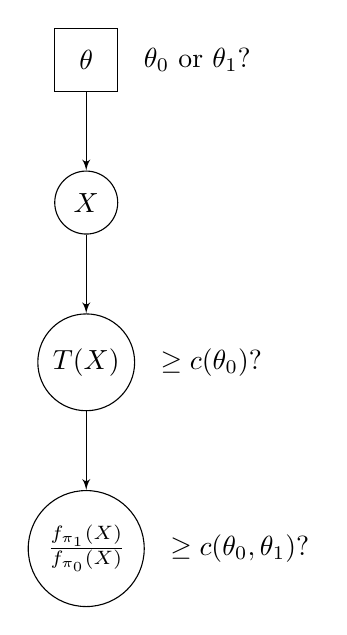
\begin{tikzpicture}[
roundnode/.style={circle, draw, minimum size=8mm},
squarenode/.style={rectangle, draw, minimum size=8mm},
vertex/.style={circle,draw,minimum size=1.5em},
edge/.style={->,> = latex'},
myblock/.style={draw}
]
%Nodes
\node[squarenode]        (theta)                            {$\theta$};
\node[roundnode]        (X)       [below=of theta]        {$X$};
\node[roundnode]        (TX)       [below=of X]        {$T(X)$};
\node[roundnode]        (lr)       [below=of TX]        {$\frac{f_{\pi_1}(X)}{f_{\pi_0}(X)}$};


%Lines
\draw[edge] (theta.south) -- (X.north);
\draw[edge] (X.south) -- (TX.north);
\draw[edge] (TX.south) -- (lr.north);

\node [rectangle, draw=none, right=0.2cm] (inv) at (theta.east) {$\theta_0$ or $\theta_1$?};
\node [rectangle, draw=none, right=0.2cm] (inv) at (TX.east) {$\geq c(\theta_0)$?};
\node [rectangle, draw=none, right=0.2cm] (inv) at (lr.east) {$\geq c(\theta_0, \theta_1)$?};

\end{tikzpicture}

\end{document}